\documentclass[11pt]{article}

\usepackage[
	left = 0.5in, 
	right = 0.5in, 
	top = 1in, 
	bottom = 1in
]{geometry}

\usepackage{amsfonts, amsmath, amssymb}

\usepackage[none]{hyphenat} %remove splitting words with hyphen

\usepackage{graphicx}

\usepackage{float}

\usepackage[nottoc, notlot, notlof]{tocbibind}

\usepackage{fancyhdr}
\pagestyle{fancy}

\fancyhead{}  %remove existing header
\fancyfoot{}  %remove existing footer

% belo L = Left, R = Right, C = Center
\fancyhead[L]{\slshape \MakeUppercase{Title }} %italisize using slshape 
\fancyhead[R]{\slshape Name Here}
\fancyfoot[C]{\thepage} % \thepage will bring pagenumber on footer

% \renewcommand{\headrulewidth}{0pt} % remove header line
\renewcommand{\footrulewidth}{0pt} % remove footer line

% \parindent 0ex % paragraphs will not be indented
% \setlength{\parindent}{4em} % specify paraindentation length
% \setlength{\parskip}{1em}	% space between paragraphs
\renewcommand{\baselinestretch}{1.5} % paragraph spacing


\begin{document}

\begin{titlepage}

\begin{center}

\vspace*{1cm} % force add vspace even if compiler refuses

\Large{\textbf{IB Mathematics SL}}

\Large{\textbf{Internal Assesment}}

% combination of vfill can be used to center the content
\vfill
\line(1, 0){400} \\[1mm] % slope of (x, y) is y/x 
\huge{\textbf{This is a Sample Title}} \\[1mm]
\large{\textbf{- This is a Sample Subtitle -}} \\[1mm]
\line(1, 0){400}
\vfill

By Student Name \\
Candidate \# \\
\today \\

\end{center}

\end{titlepage}

% requires tocbibind package with optional params
\tableofcontents  % automatically populate table of contents from sections
\thispagestyle{empty} % remove page number on the current page
\clearpage % put table of contents in a single page

\setcounter{page}{1} % start numbering pages from next page onwards

\section{Introduction}

In today's rapidly evolving world, it is imperative to understand the nuances of effective communication and personal engagement\footnote{An example footnote}

\section{Scoring Criteria}

\subsection{Communication}

Effective communication is not just about conveying a message, but ensuring that it is understood in its intended context. The scoring for this criterion evaluates clarity, coherence, and the appropriate use of technical terms. 

\subsection{Personal Engagement}

Personal engagement goes beyond mere participation. It assesses an individual's passion, commitment, and proactive involvement in a task or project (See table \ref{table_functions})

\begin{table}[H]
	\centering

	\begin{tabular}{|c|c|c|c|} \hline
		$ x $   & 0 & 1 & 2\\ \hline
		$ f(x)$ & 3 & 6 & 9\\ \hline
	\end{tabular}
	\caption{Caption goes here}
	\label{table_functions}
\end{table}

Personal engagement goes beyond mere participation. It assesses an individual's passion, commitment, and proactive involvement in a task or project.

\begin{figure}[H]
	\centering
	
	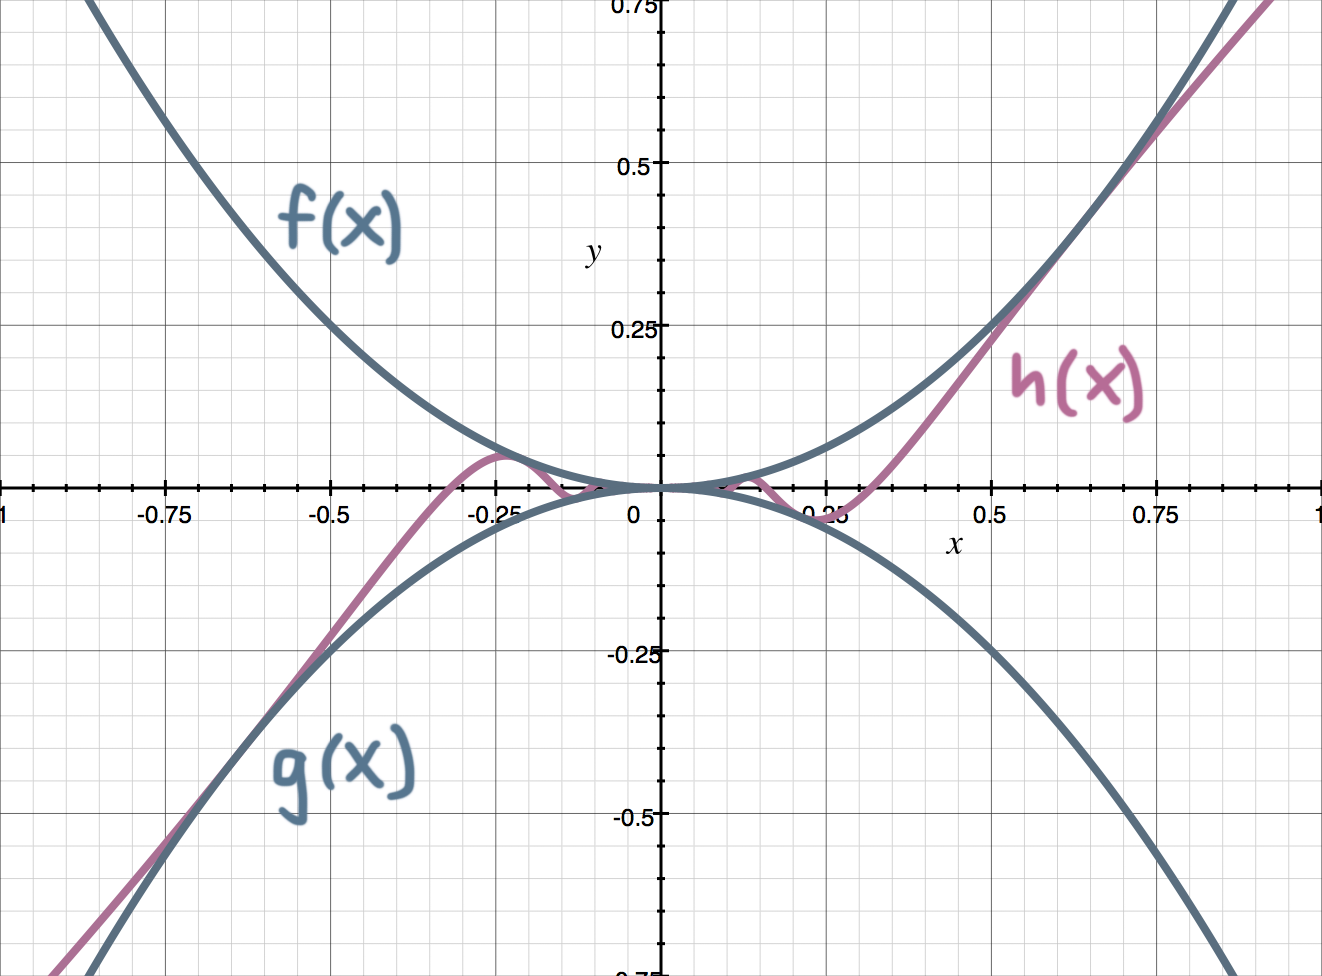
\includegraphics[width=0.5\textwidth]{limit}
	\caption{The squeeze theorem}

\end{figure}

\section{Conclusion}

To thrive in any professional or personal setting, mastering the art of communication and demonstrating genuine personal engagement are crucial. \cite{ref_diamond_bar_school}

\pagebreak
\begin{thebibliography}{}

\bibitem{ref_diamond_bar_school}
Alcosser, Howard. 
"Diamond Bar High School"
Web. 27 May 2015.
\textit{http://www.diamondbarschool.com/2014/rub.pdf}

\bibitem{ref_mybook_of_parasites}
Lastname, Firstname.
\textit{Title of Book}
City of Publication
Publisher,
Year of Publication.
Medium of publication

\end{thebibliography}

\end{document}














